\section{Auswertung}
Die im Versuch verwendeten Bauelemente (siehe \eqref{eq: bauteile})
werden als fehlerfrei angenommen.
Hingegen ist der veränderbare Kondensator $C\ua{k}$ mit
einem relativen Fehler von $20\,\%$ behaftet.
Die resultierenden Fehler werden mit der Python Bibliothek 
\emph{uncertainties} bestimmt.

\subsection{Bestimmung des Verhältnisses von Schwingungs- und Schwebungsfrequenz}
Die bei verschieden eingestellten $C\ua{k}$ gezählten Schwingungsmaxima pro einer halben
Schewbungsperiode (einem 'Bauch') werden in Tabelle \ref{fig:teila_n_ck} aufgelistet.
Zusätzlich befindet sich in der Tabelle, das Verhältnis zur Schwebungsperiode.
Bestimmt wurde diese mittels
\begin{equation*}
n=\frac{1}{\mathup{Anzahl der Schwingungsmaxima}}
\end{equation*}
\begin{table} 
\centering 
\caption{ Anzahl der Schwingungsmaxima bei verschiedenenen Kapazitäten $C_k$} 
\label{teila_n_ck} 
\begin{tabular}{S S } 
\toprule  
{$C_k in $\si{\nano\farad}$} & {Anzahl der Schwingungsmaxima}  \\ 
\midrule  
 \num{1.0+/-0.2}  & \num{1.0+/-1.0}\\ 
\num{2.2+/-0.4}  & \num{1.0+/-1.0}\\ 
\num{2.7+/-0.5}  & \num{2.0+/-1.0}\\ 
\num{4.7+/-0.9}  & \num{2.0+/-1.0}\\ 
\num{6.8+/-1.4}  & \num{3.0+/-1.0}\\ 
\num{8.2+/-1.6}  & \num{3.0+/-1.0}\\ 
\num{10.0+/-2.0}  & \num{4.0+/-1.0}\\ 
\num{12.0+/-2.4}  & \num{5.0+/-1.0}\\ 
\bottomrule 
\end{tabular} 
\end{table}

\subsection{Bestimmung der theoretischen Fundamentalfrequenzen}
Um die theoretischen Fundamentalfrequenzen zu bestimmen, werden die Gleichungen \eqref{eq: nu+} und 
\eqref{eq: nu-} verwendetet.
Für die erste Fundamentalfrequenz (gleichphasiges Schwingen) ergibt sich der 
theoretische Wert

\begin{equation}
\label{eq:nu_plu_theo}
\nu_{+\,\mathup{theo}}=\SI{36,5}{\kilo\hertz}.
\end{equation}
Und für die gegenphasigen Fundamentalfrequenzen ergibt sich in Abhängigkeit von $C\ua{k}$ die in Tabelle \ref{fig:teilb_frequenzen_theo} zu dargestellten Werte. 
\begin{table}
\centering
\caption{Theoretisch bestimmte Fundamentalfrequenzen}
\label{fig:teilb_frequenzen_theo}
\begin{tabular}{S S }
\toprule
{$C\ua{k}$ in $\si{\nano\farad}$} &{$\nu_{-\,\mathup{theo}}$ in $\si{\kilo\hertz}$}  \\ 
\midrule
 \num{1.0\pm0.2} & \num{58.7\pm3.6}\\
\num{2.2\pm0.4} & \num{47.9\pm2.0}\\
\num{2.7\pm0.5} & \num{46.0\pm1.7}\\
\num{4.7\pm0.9} & \num{42.2\pm1.1}\\
\num{6.8\pm1.4} & \num{40.5\pm0.8}\\
\num{8.2\pm1.6} & \num{39.9\pm0.6}\\
\num{10.0\pm2.0} & \num{39.3\pm0.5}\\
\num{12.0\pm2.4} & \num{38.9\pm0.5}\\
\bottomrule
\end{tabular}
\end{table}


\subsection{Bestimmung der Fundamentalfrequenzen mithilfe erzwungener Schwingungen}
Die bei verschieden eingestellten $C\ua{k}$ bestimmten Fundamentalfrequenzen 
$\nu_+$ und $\nu_-$
sind in Tabelle \ref{fig:teilb_schwingungen_prak_theo} zu finden.
Zusätzlich ist in der Tabelle das Verhältnis der gemessenen Frequenzen 
zu den theoretisch errechneten Frequenzen dargestellt.
Die Verhältnisse werden mit
\begin{equation}
\label{eq:verh}
n_+=\frac{\nu_+}{\nu_{+\,\mathup{theo}}} \qquad n_-=\frac{\nu_-}{\nu_{-\,\mathup{theo}}}
\end{equation}
berechnet.
\FloatBarrier
\begin{table}
\centering
\caption{ Gemessene Fundamentalfrequenzen bei einer erzwungenen Schwingungen und das relative Verhältnis zu den Theoriewerten}
\label{fig:teilb_schwingungen_prak_theo}
\begin{tabular}{S S S S S }
\toprule
{$C\ua{k}$ in $\si{\nano\farad}$} & {Frequenz $\nu_-$ in $\si{\kilo\hertz}$} & {Frequenz $\nu_+$ in $\si{\kilo\hertz}$}& {rel. Abw. $n_-$ in \%} & {rel. Abw. $n_+$ in \%}  \\ 
\midrule
 \num{1.0\pm0.2} & \num{76.9\pm1.0} & \num{33.3\pm1.0} & \num{31.0\pm8.2} & \num{-8.7\pm2.7}\\
\num{2.2\pm0.4} & \num{62.5\pm1.0} & \num{33.3\pm1.0} & \num{30.5\pm5.9} & \num{-8.7\pm2.7}\\
\num{2.7\pm0.5} & \num{55.8\pm1.0} & \num{32.3\pm1.0} & \num{21.3\pm5.0} & \num{-11.6\pm2.7}\\
\num{4.7\pm0.9} & \num{47.6\pm1.0} & \num{33.3\pm1.0} & \num{12.8\pm3.7} & \num{-8.9\pm2.7}\\
\num{6.8\pm1.4} & \num{43.5\pm1.0} & \num{33.3\pm1.0} & \num{7.2\pm3.2} & \num{-8.7\pm2.7}\\
\num{8.2\pm1.6} & \num{41.7\pm1.0} & \num{32.3\pm1.0} & \num{4.5\pm3.0} & \num{-11.6\pm2.7}\\
\num{10.0\pm2.0} & \num{40.0\pm1.0} & \num{33.3\pm1.0} & \num{1.8\pm2.9} & \num{-8.7\pm2.7}\\
\num{12.0\pm2.4} & \num{38.6\pm1.0} & \num{33.3\pm1.0} & \num{-0.5\pm2.8} & \num{-8.7\pm2.7}\\
\bottomrule
\end{tabular}
\end{table}

\FloatBarrier
In Abbildung \ref{fig: plot} sind die Messwerte grraphisch dargestellt.

\subsection{Bestimmung der Fundamentalfrequenzen mithilfe der Sweep-Methode}
Zunächst werden die Grundeinstellungen des Sweeps besprochen.
Die Periodendauer eines Sweepes beträgt $P=\SI{1}{\second}$.
Die Startfrequenz ist $\nu\ua{sta}=\SI{15.67}{\kilo\hertz}$ und die
Endfrequenz liegt bei $\nu\ua{end}=\SI{96.15}{\kilo\hertz}$.
Aufgrund einer linearen Erhöhung der Frequenz kann eine Geradengleichung ermittelt werden. 
Mit dieser kann zu jedem Zeitpunkt ($t\in\left[0,1\right)\,\si{\second}$) auf die Frequenz geschlossen werden.
Für die Parameter der Geradengleichung ergeben sich:

\begin{equation*}
b=\SI{15.7}{\kilo\hertz} \qquad m=\frac{\nu\ua{end}-\nu\ua{sta}}{P}=\SI{80.5}{\kilo\hertz\per\second}
\end{equation*}
Insgesamt folgt dann für die Gleichung

\begin{equation}
\label{eq:geraden}
g(t)=mt+b=80.5\,t+15.7
\end{equation}

Die im Versuch gemessenen Zeitabstände sind in Tabelle \ref{fig:teilc_gemessene_zeit} dargestellt.
\begin{table} 
\centering 
\caption{Gemessene Zeitabstände bei unterschiedlichen $C\ua{k}$} 
\label{teilc_gemessene_zeit} 
\begin{tabular}{S S S } 
\toprule  
{$C\ua{k}$ in $\si{\nano\farad}$} & {Abstand $\Delta t_+$} & {Abstand $\Delta $}  \\ 
\midrule  
 \num{1.0\pm0.2} & \num{792.0\pm5.0} & \num{212.0\pm5.0}\\ 
\num{2.2\pm0.4} & \num{552.0\pm5.0} & \num{212.0\pm5.0}\\ 
\num{2.7\pm0.5} & \num{492.0\pm5.0} & \num{212.0\pm5.0}\\ 
\num{4.7\pm0.9} & \num{396.0\pm5.0} & \num{216.0\pm5.0}\\ 
\num{6.8\pm1.4} & \num{352.0\pm5.0} & \num{212.0\pm5.0}\\ 
\num{8.2\pm1.6} & \num{328.0\pm5.0} & \num{216.0\pm5.0}\\ 
\num{10.0\pm2.0} & \num{308.0\pm5.0} & \num{216.0\pm5.0}\\ 
\num{12.0\pm2.4} & \num{292.0\pm5.0} & \num{212.0\pm5.0}\\ 
\bottomrule 
\end{tabular} 
\end{table}


Mithilfe von Formel \eqref{eq:geraden} können nun die Frequenz bestimmt werden (siehe Tabelle \ref{fig:teilc_schwingungen_prak_theo}.
Äquivalent zu Formel \eqref{eq:verh} wurden die in Tab. \ref{fig:teilc_schwingungen_prak_theo} angebenden Verhältnisse berechnet.
\begin{table} 
\centering 
\caption{ Bestimmung der Fundamentalfrequenzen mit der 'Sweep-Methode' und zusätzlich das Verhältnis zu den Theoriewerten} 
\label{fig:teilc_schwingungen_prak_theo} 
\begin{tabular}{S S S S S } 
\toprule  
{$C\ua{k}$ in $\si{\nano\farad}$} & {Frequenz $\nu_-$ in $\si{\kilo\hertz}$} & {Frequenz $\nu_+$ in $\si{\kilo\hertz}$ }& {Verhältnis $n_-$} & {Verhältnis $n_+$}  \\ 
\midrule  
 \num{1.0\pm0.2} & \num{79.4\pm0.4} & \num{32.7\pm0.4} & \num{1.4\pm0.1} & \num{0.9\pm0.0}\\ 
\num{2.2\pm0.4} & \num{60.1\pm0.4} & \num{32.7\pm0.4} & \num{1.3\pm0.1} & \num{0.9\pm0.0}\\ 
\num{2.7\pm0.5} & \num{55.3\pm0.4} & \num{32.7\pm0.4} & \num{1.2\pm0.0} & \num{0.9\pm0.0}\\ 
\num{4.7\pm0.9} & \num{47.5\pm0.4} & \num{33.1\pm0.4} & \num{1.1\pm0.0} & \num{0.9\pm0.0}\\ 
\num{6.8\pm1.4} & \num{44.0\pm0.4} & \num{32.7\pm0.4} & \num{1.1\pm0.0} & \num{0.9\pm0.0}\\ 
\num{8.2\pm1.6} & \num{42.1\pm0.4} & \num{33.1\pm0.4} & \num{1.1\pm0.0} & \num{0.9\pm0.0}\\ 
\num{10.0\pm2.0} & \num{40.5\pm0.4} & \num{33.1\pm0.4} & \num{1.0\pm0.0} & \num{0.9\pm0.0}\\ 
\num{12.0\pm2.4} & \num{39.2\pm0.4} & \num{32.7\pm0.4} & \num{1.0\pm0.0} & \num{0.9\pm0.0}\\ 
\bottomrule 
\end{tabular} 
\end{table}
Die Messwerte in der Abbildung \ref{fig: plot} einmal aufgetragen.
\begin{figure}
  \centering
  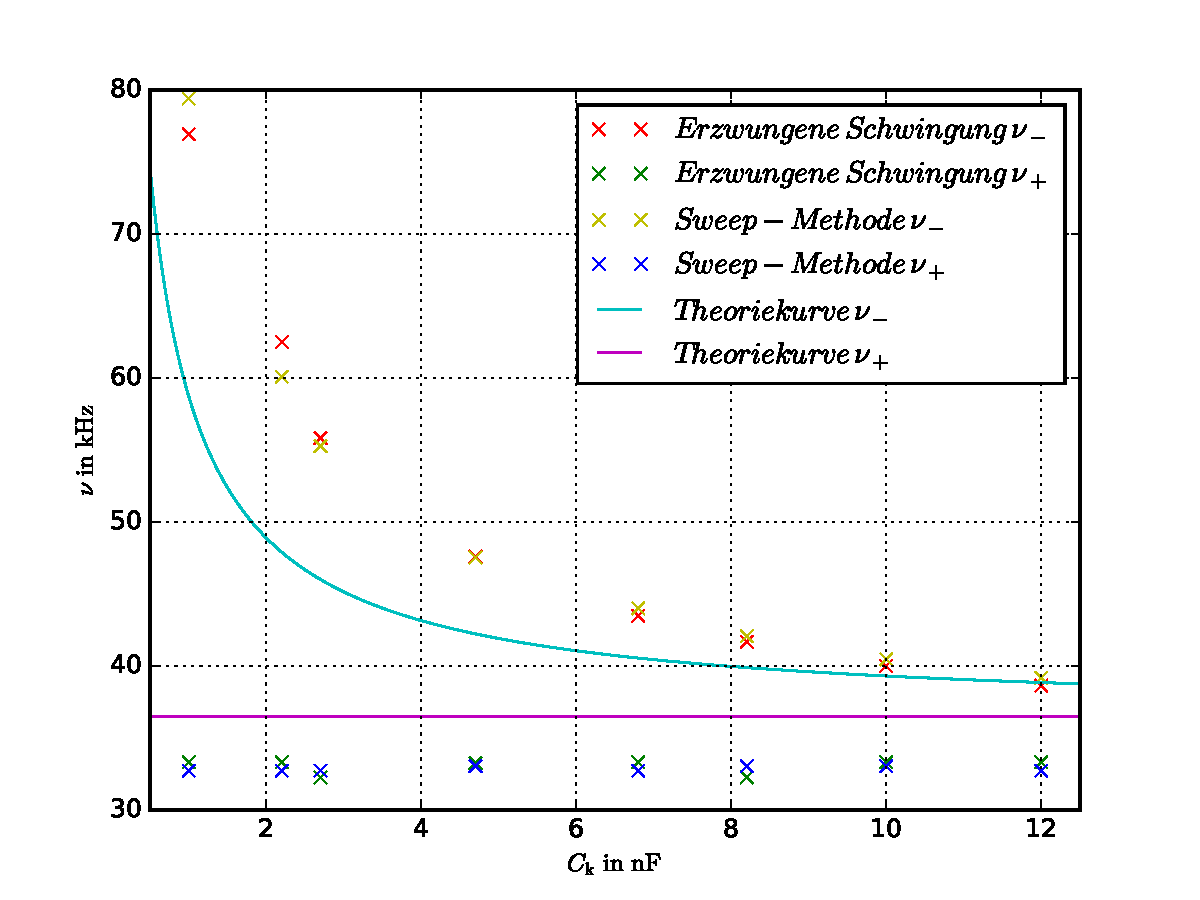
\includegraphics[width=0.8\textwidth]{pics/plot_frequenzen.pdf}
  \caption{Darstellung der Frequenzen in Abhängigkeit der verschiedenen $C\ua{k}$}
  \label{fig: plot}
\end{figure}